Algorithmic Music Composition (AMC) can be literally defined as the use of algorithms to compose music. This broad term includes non computational procedures from music theory developed to guide music composition and computational methods designed to generate music automatically or semi-automatically. This chapter presents a brief history of AMC to contextualize this dissertation, from the first procedures created by medieval music theorists to the modern computational methods designed by scientists and engineers. Most computational methods are briefly discussed with a few examples in this chapter, except neural networks, which are covered in greater detail in the next chapter. Moreover, it is important to highlight that this dissertation focuses on symbolic music composition, and hence audio-based methods are not covered in these chapters.

\section{Procedures in Music Theory}

% Guido of Arezzo
Music composers have been developing procedures for centuries to compose different aspects of music pieces. Guido of Arezzo (around 991-–1031), in his work \textit{Micrologus}, describes a method for mapping Latin lyrics into melodies. The method extracts the vowels from given Latin lyrics and then maps the vowels into pitches. Figure \ref{fig:arezzo} shows this procedure considering the seven different natural pitches of the western music system\footnote{C, D, E, F, G, A, B}. Since there are more pitches than vowels, some vowels are mapped to different pitches. When mapping vowels that have more than one associated pitch, the pitch should be selected at random. For example, consider this verse from the \textit{Hymn to St John} with the extracted vowels in parenthesis:

% \poemtitle{Fleas}
\settowidth{\versewidth}{UT queant laxis,}
\begin{verse}[\versewidth]
    REsonare fibris (eoaeii) \\
    MIra gestorum (iaeou) \\
    FAmuli tuorum (auiuou) \\
    SOLve polluti (oeoui)\\
    LAbii reatum  (aiieau)\\
    Sancte Ioannes (aeioae)
\end{verse}

Using the mapping rules defined in Figure \ref{fig:arezzo}, the first line of the verse can
be mapped to the melody \textit{D, B, F, C, C, E}.

\begin{figure}[!h]
 \centering
 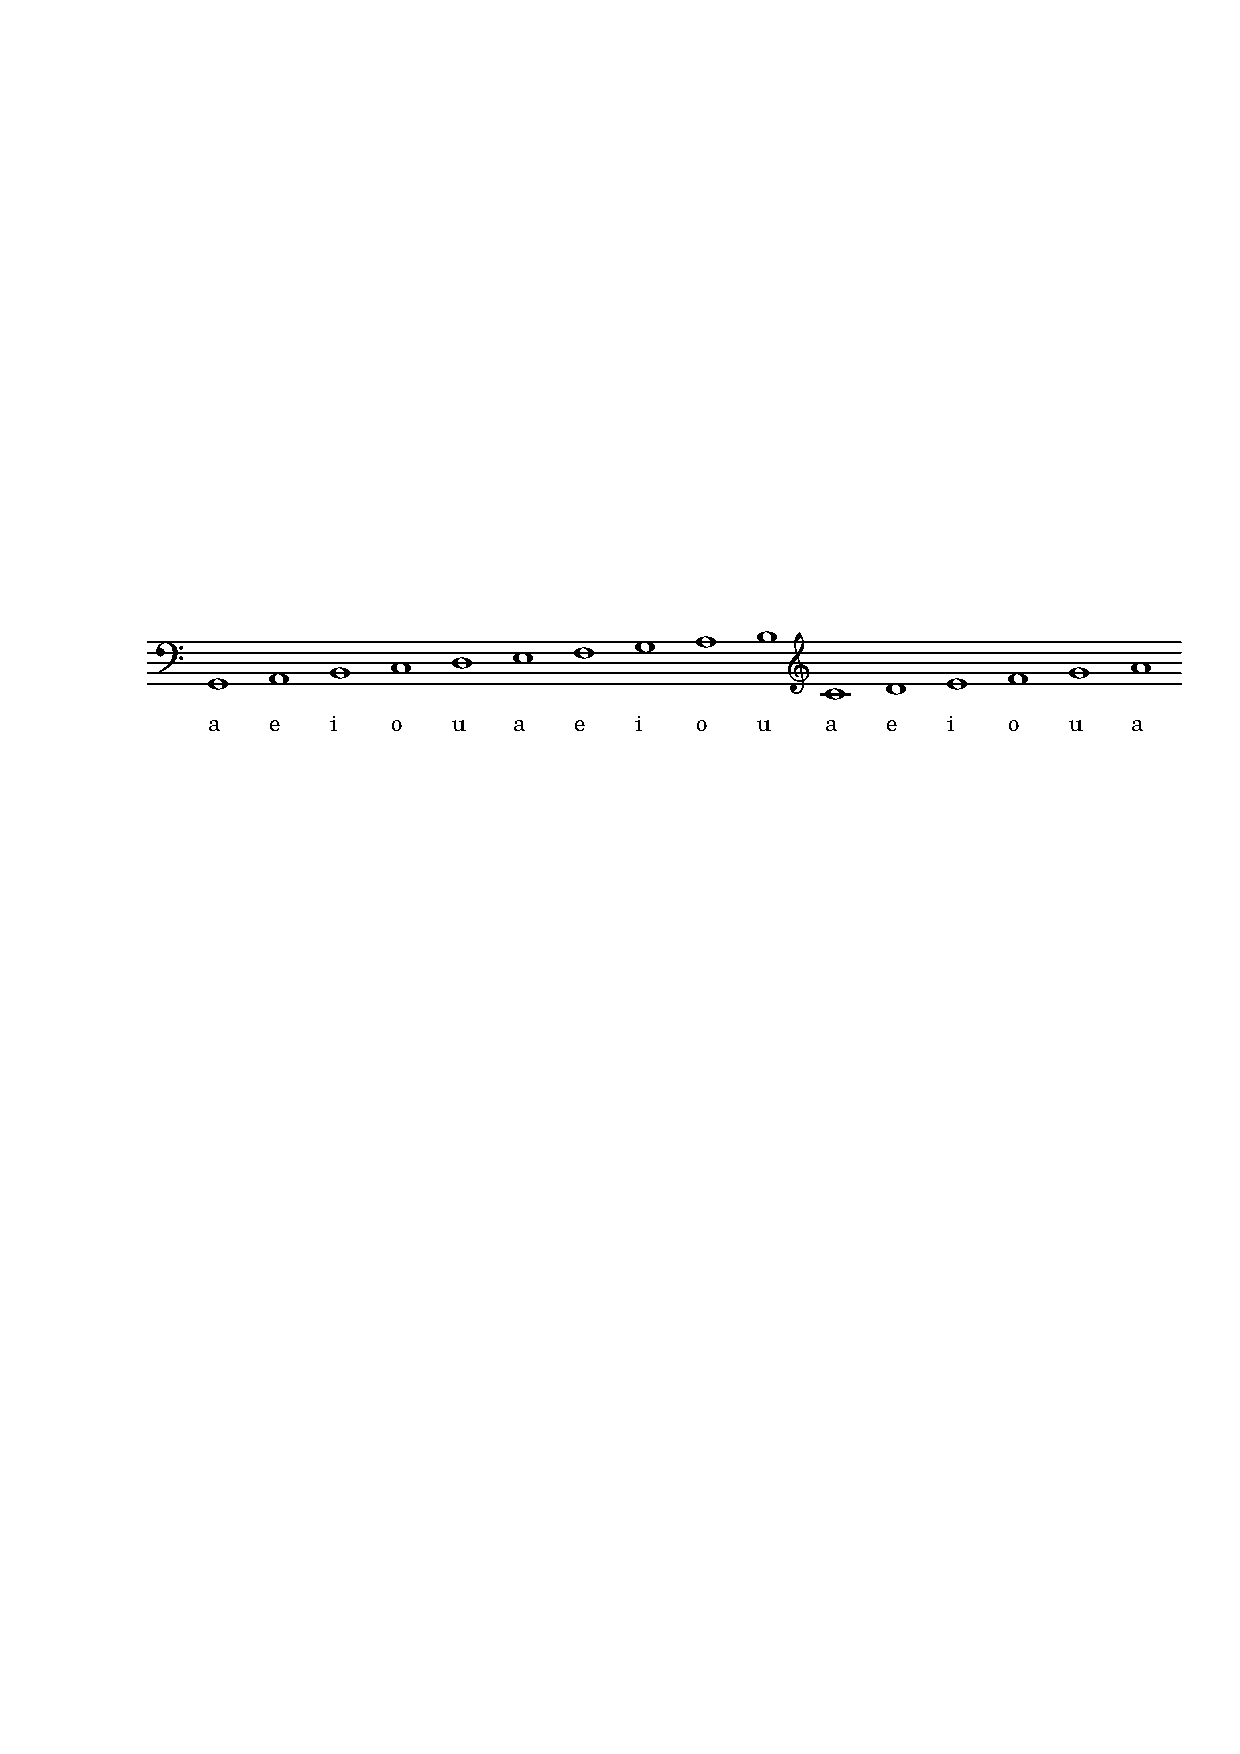
\includegraphics[width=\columnwidth]{imgs/background/arezzo.pdf}
 \caption{Mapping of vowels on tone pitches by Guido of Arezzo.}
 \label{fig:arezzo}
\end{figure}

% Isorhythm
Around 1280, the music theorist Franco de Cologne, in his work \textit{Cantus Mensurabilis}, introduced a music notation system where the note durations are defined by their shapes. This new notation allowed
composers to treat rhythm independently of the pitch. For example, French composers of the \textit{ars nova}, such as Phillipe de Vitry and Guillaume de Machaut, used a technique called isorhythm to map a rhythmic pattern (named the \textit{talea}) onto a pitch contour (named the \textit{color}). Figure \ref{fig:isorhythm} shows the tenor melody of the piece \textit{De bon espoir-Puisque la douce-Speravi} by Guillaume de Machaut built using the isorhythm technique.

\begin{figure}[!h]
 \centering
 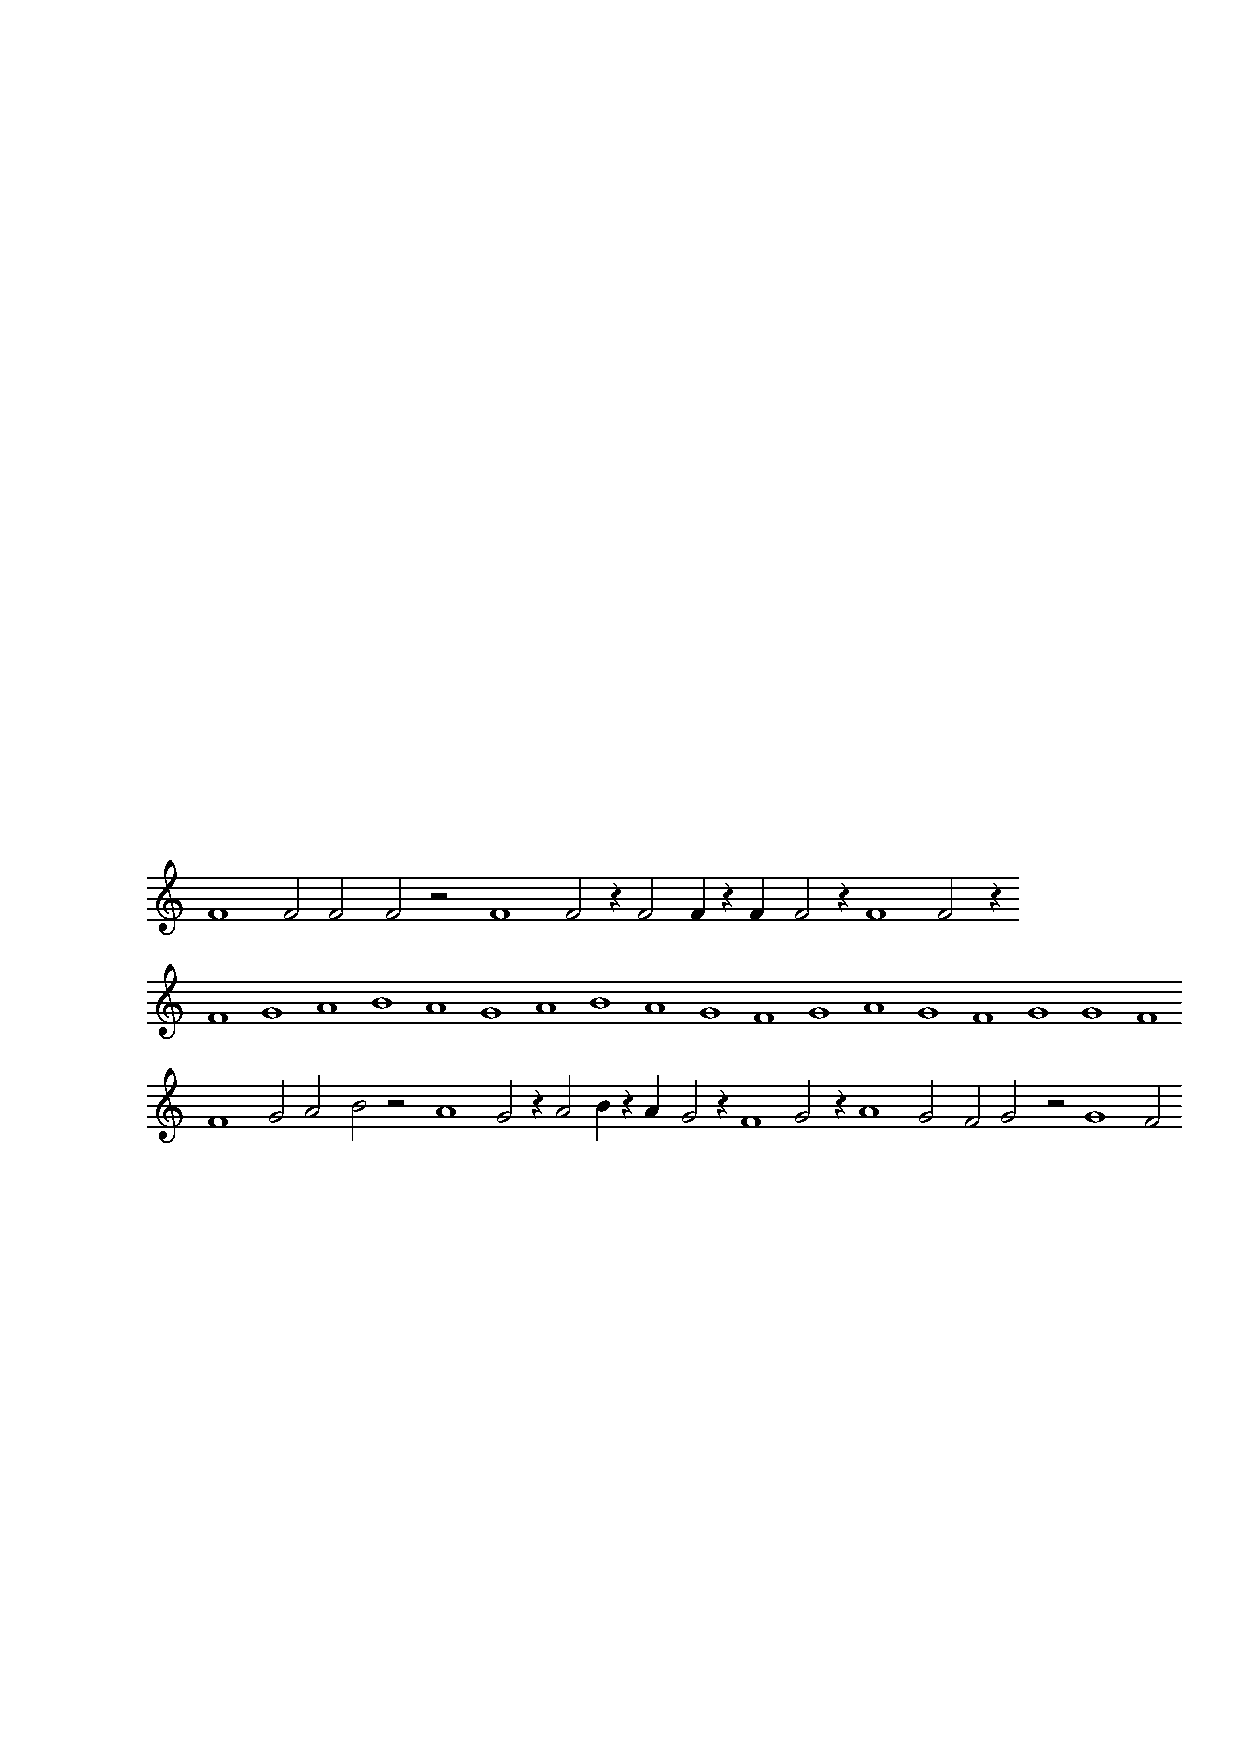
\includegraphics[width=\columnwidth]{imgs/background/isorhythm.pdf}
 \caption{The tenor of \textit{De bon espoir-Puisque la douce-Speravi} by Guillaume de Machaut.}
 \label{fig:isorhythm}
\end{figure}

The first staff is the talea and the second one is the color. The third staff is the resulting piece of applying the former onto the latter. In this example, the talea has twelve notes and five rests, whereas the color has eighteen notes. The note durations of the talea are applied in order onto the respective notes of the color. Whenever there is a rest in the talea, that rest is merged into the pitches of the color. If the last note of the talea is mapped and there are still notes left in the color, the mapping process continues from the first note of the talea.

% Counterpoint: Art of Fugue
In the Baroque Period (1600--1750), Johann Sebastian Bach wrote \textit{The Art of Fugue}, a musical
work that explores different fugues and cannons from a single musical subject. Fugues
and cannons are highly procedural forms of contrapuntal compositional techniques.
Counterpoint consists of interleaving two or more melodies that are harmonically
dependent but independent in rhythm and melodic contour. In a canon, the composer starts
with a melody, called the \textit{leader}, which is strictly followed at a delayed time interval
by another voice, called the \textit{follower}. The follower may present a variation of the leader
through transformation operations such as transposition\footnote{Moving a set of notes up or down
in pitch by a constant interval}, augmentation\footnote{Repeating a set of notes with longer durations.}, or inversion\footnote{Playing a given set of notes upside down, reversing the contour of the notes.} \cite{simoni2003algorithmic}. Figure \ref{fig:canon} shows the first twelve measures of the
canon named \textit{Canon per Augmentationem in Contrario Motu} from \textit{The Art of Fugue}.

\begin{figure}[!h]
 \centering
 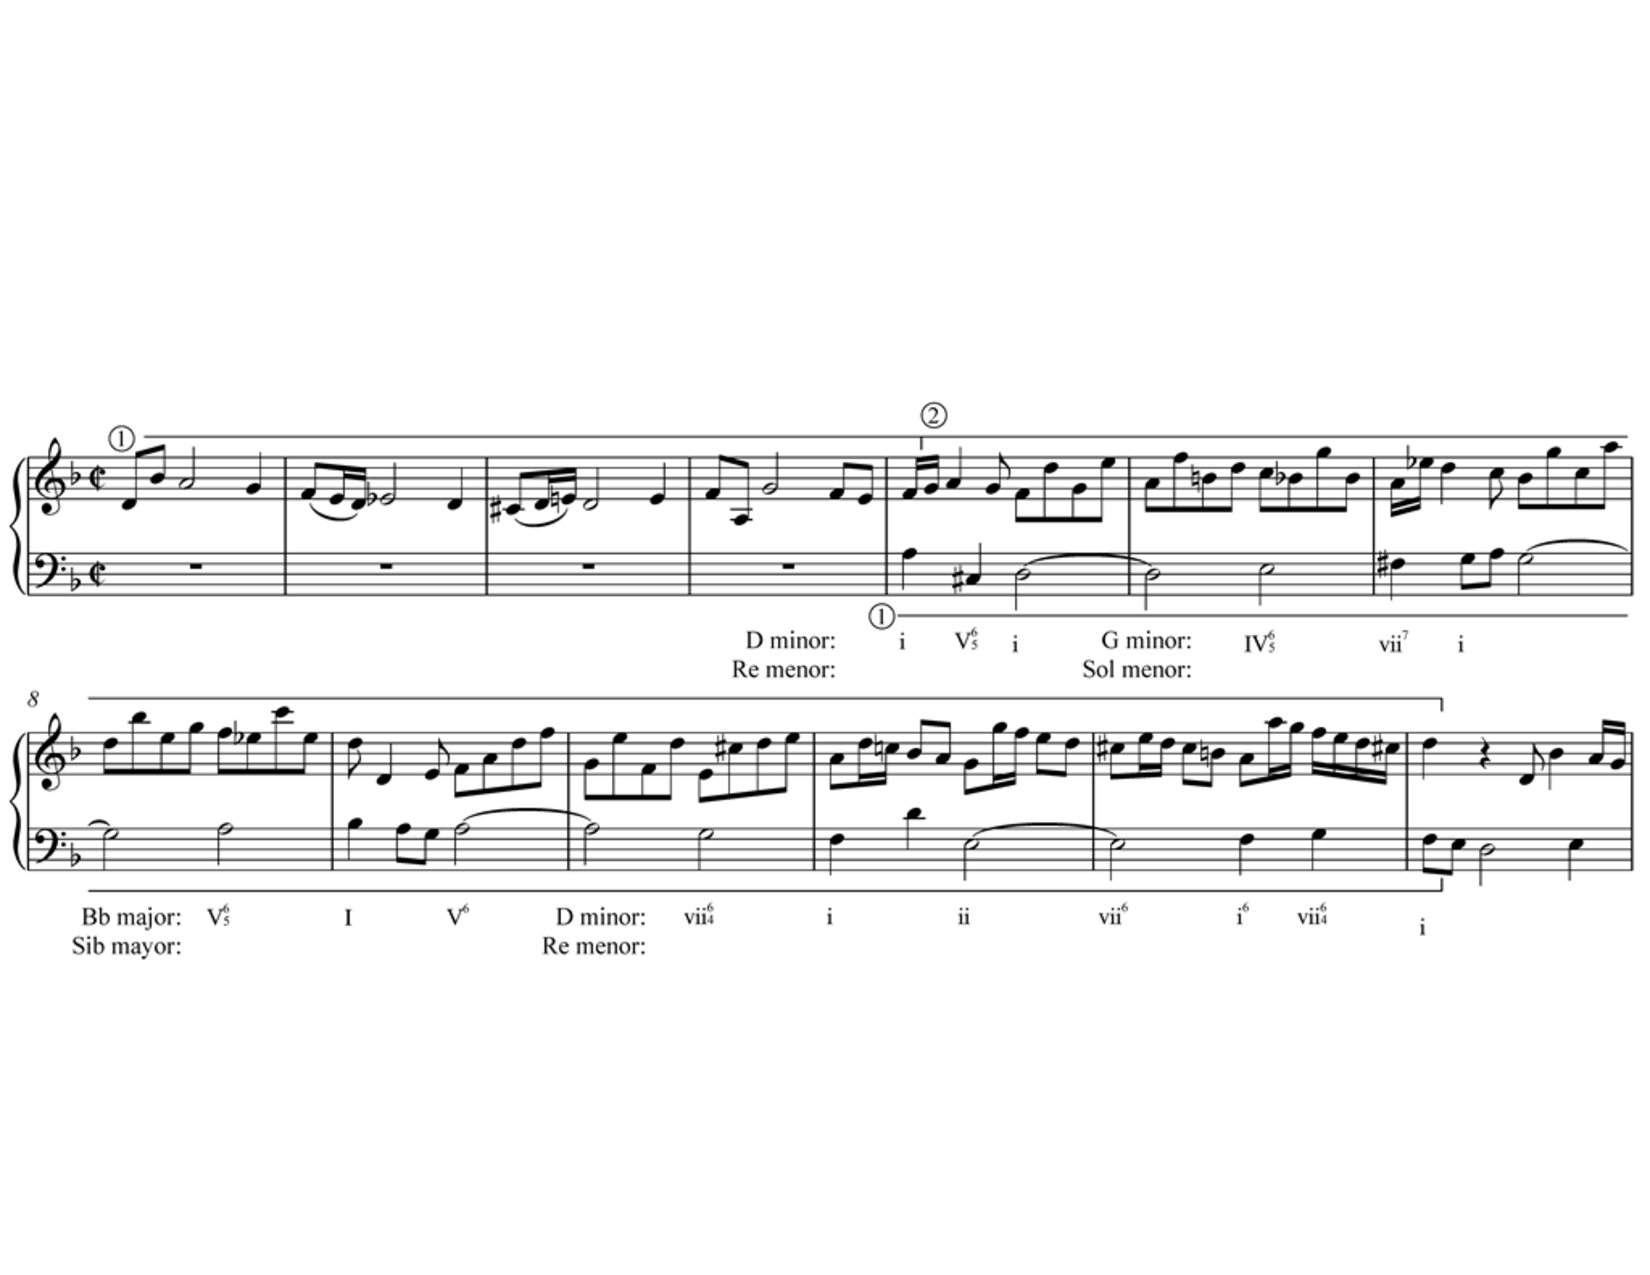
\includegraphics[width=\columnwidth]{imgs/background/canon_a.pdf}
 \caption{\textit{Canon per Augmentationem in Contrario Motu} from \textit{The Art of the Fugue} by Johann Sebastian Bach.}
 \label{fig:canon}
\end{figure}

Figure \ref{fig:canon_subject} shows the follower voice (measures 5 to 13) transforming the leader
(measures 1 to 5) using augmentation and inversion. The follower voice, due to augmentation, needs eight
measures to answer the first four measures.

\begin{figure}[!h]
 \centering
 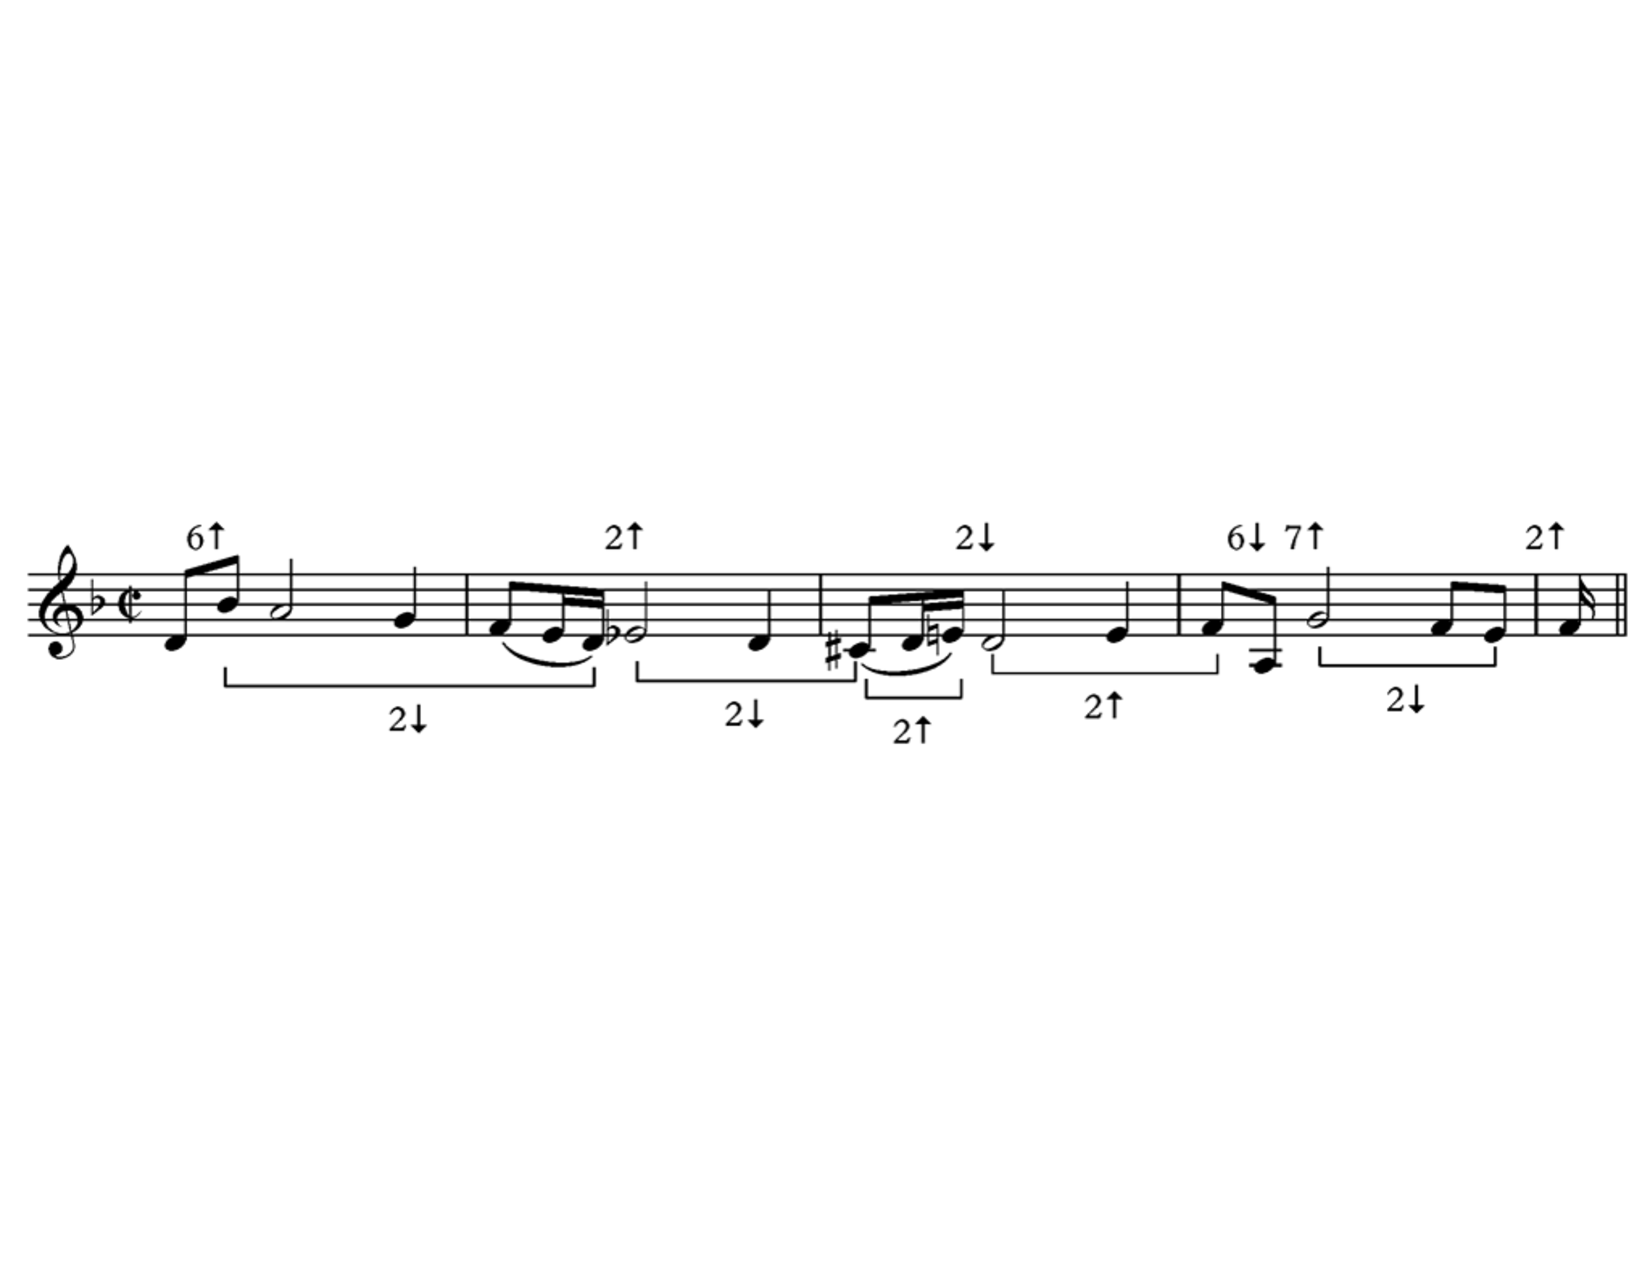
\includegraphics[width=\columnwidth]{imgs/background/canon_b.pdf}
 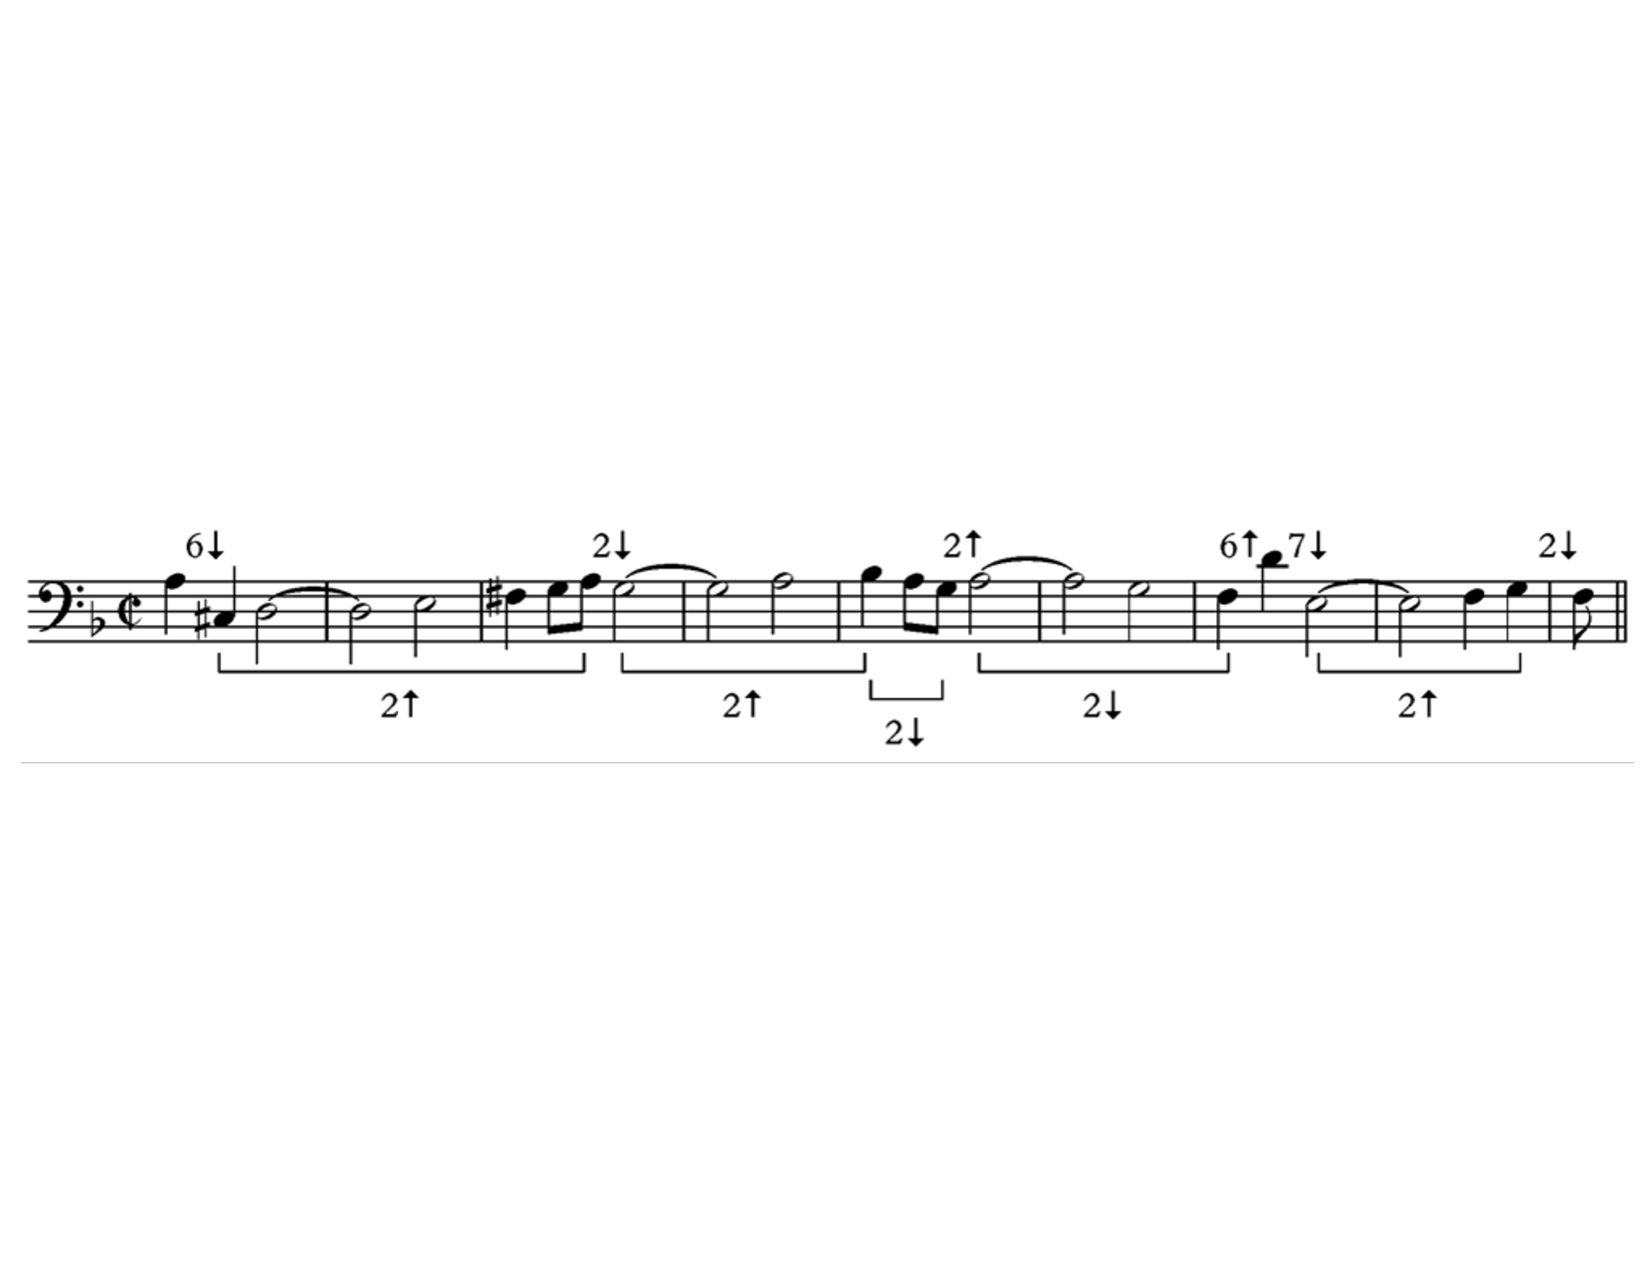
\includegraphics[width=\columnwidth]{imgs/background/canon_c.pdf}
 \caption{Subject of the canon.}
 \label{fig:canon_subject}
\end{figure}

% Mozart's dice game
In the Classical Period (1750-1827), \textit{Musikalisches Würfelspie} (german for a musical dice game) became a popular method to generate music randomly. It consists of selecting precomposed snippets of music according to the result of dice rolls. One of the most famous applications of this method is attributed to Wolfgang Amadeus Mozart, although this attribution has not been authenticated \cite{cope1989experiments}. Mozart's dice game was designed to generate sixteen-measure-long minuets\footnote{A minuet is a classic form of dance from the classical period.}. The game works by creating an eleven-by-sixteen table, where the rows represent possible results of rolling two six-sided dice and columns are the indices of each measure of the minuet. Each element in the table is a precomposed measure. Table \ref{tab:mozart_dice} shows an example of Mozart's dice game with only the first part of the minuet and hence only eight columns.

\begin{table}[h]
    \centering
    % \setlength{\tabcolsep}{4pt}
    \begin{tabular}{ccccccccc}
    \toprule
    & \multicolumn{8}{c}{\textbf{Part 1}} \\
    & I & II & III & IV & V & VI & VII & VII \\
    \midrule
    2  & 96  & 22  & 141 & 41  & 105 & 122 & 11  & 30  \\
    3  & 32  & 6   & 128 & 63  & 146 & 46  & 134 & 81  \\
    4  & 69  & 95  & 158 & 13  & 153 & 55  & 110 & 24  \\
    5  & 40  & 17  & 113 & 85  & 161 & 2   & 159 & 100 \\
    6  & 148 & 74  & 163 & 45  & 80  & 97  & 36  & 107 \\
    7  & 104 & 157 & 27  & 167 & 154 & 68  & 118 & 91  \\
    8  & 152 & 60  & 171 & 53  & 99  & 133 & 21  & 127 \\
    9  & 119 & 84  & 114 & 50  & 140 & 86  & 169 & 94  \\
    10 & 98  & 142 & 42  & 156 & 75  & 129 & 62  & 123 \\
    11 & 3   & 87  & 165 & 61  & 135 & 47  & 147 & 33  \\
    12 & 54  & 130 & 10  & 103 & 28  & 37  & 106 & 5   \\
    \bottomrule
    \end{tabular}
    \caption{Example of Mozart's dice game. Each element in the table is an integer
    representing the number of a pre-composed measure.}
    \label{tab:mozart_dice}
\end{table}

To generate the first part of the minuet with this implementation, one has to roll two six-sided dice
for each column $j$ of the Table \ref{tab:mozart_dice}. After each roll, the sum $i$  of the two dice is
used to look up the row number $i$ for column $j$. The element $i,j$ in the Table \ref{tab:mozart_dice}
is then used to retrieve a single measure from a collection of musical fragments.
Figure \ref{fig:mozart_dice} shows the first eight measures of a minuet that can
be generated using the Table \ref{tab:mozart_dice}.

\begin{figure}[!h]
 \centering
 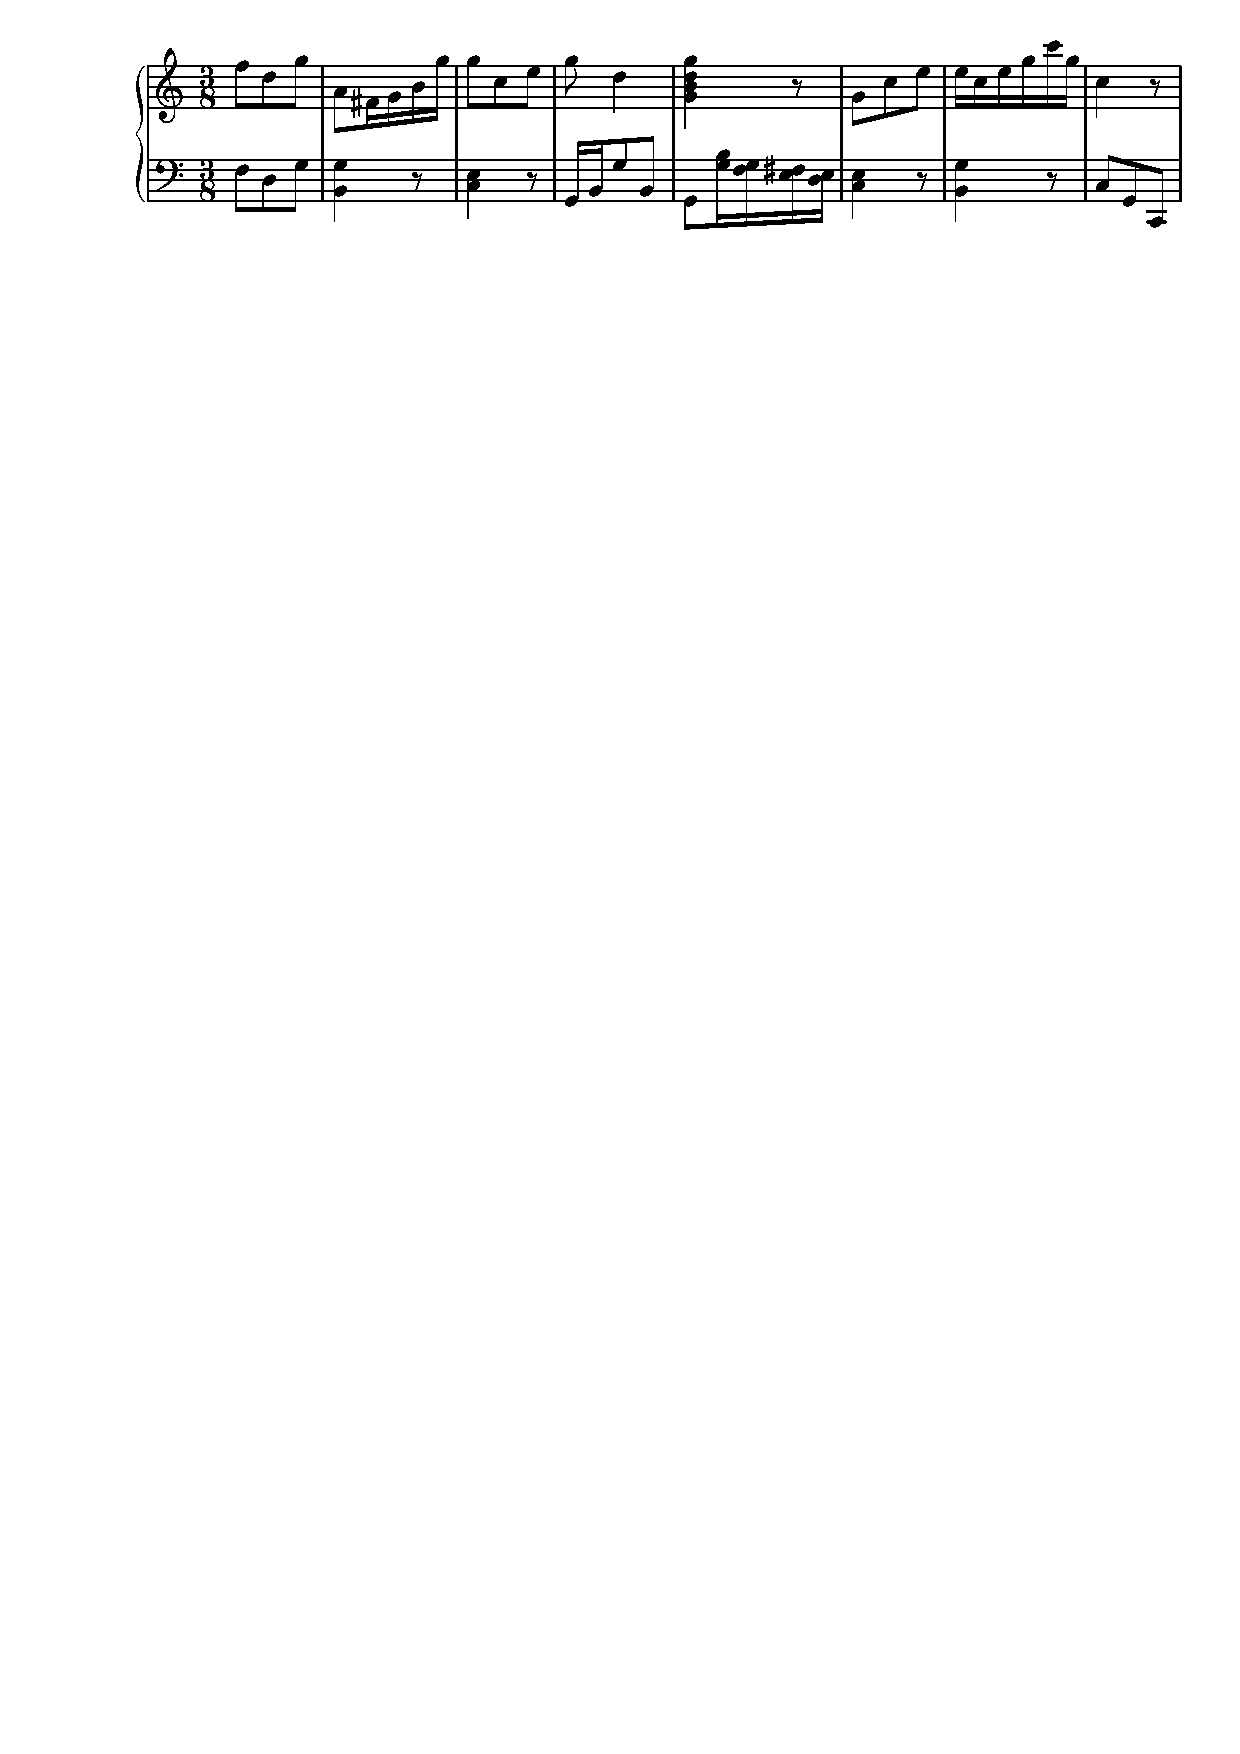
\includegraphics[width=\columnwidth]{imgs/background/mozart_dice.pdf}
 \caption{Example of minuet generated using Mozart's dice game.}
 \label{fig:mozart_dice}
\end{figure}

% Schoenberg's twelve-tone
In the Romantic Period (1800--1850), composers developed a harmonic vocabulary with extensive use of chromaticism\footnote{Chromaticism is the use of notes outside the scale of which a composition is based.}. In the transition from Romanticism to Modernism, Arnold Schoenberg, with his students, Anton Webern and Alban Berg, established new procedures for music composition called \textit{Twelve-tone serialism}. Serial composition consists of arranging a series (or row) of musical elements (such as pitches, rhythms, dynamics, timbres, and others) into a pattern that repeats itself throughout a composition.

A basic form of serial composition consists of selecting a given number of notes on the chromatic
scale\footnote{A musical scale with twelve pitches, each a semitone, above or below its adjacent pitches.}
and creating permutations using only that number of notes. The selected notes, called the \textit{row},
must all be played once before repeating, although a note can be repeated immediately after it has been
played (for example, A, and then A). The first arrangement of the row is called the \textit{tone row}.
Transformations such as transposition, inversion, retrograde\footnote{Playing a sequence of notes backwards.}
or retrograde inversion\footnote{Playing a sequence of notes backwards and upside down.} can be applied to
the tone to introduce variation into a serial composition. \textit{Twelve-tone serialism} is a serial
technique where the tone row is an ordered arrangement of the twelve notes of the chromatic scale.
The goal of this technique was to replace tonal music, which is built based on keys (such as C major or D
minor). By focusing on the twelve notes of the chromatic scale, no emphasis is given to any single key.
Figure \ref{fig:serial} illustrates the tone row used by Alban Berg in the \textit{Lyric Suite} for string
quartet composed in 1926.

\begin{figure}[!h]
 \centering
 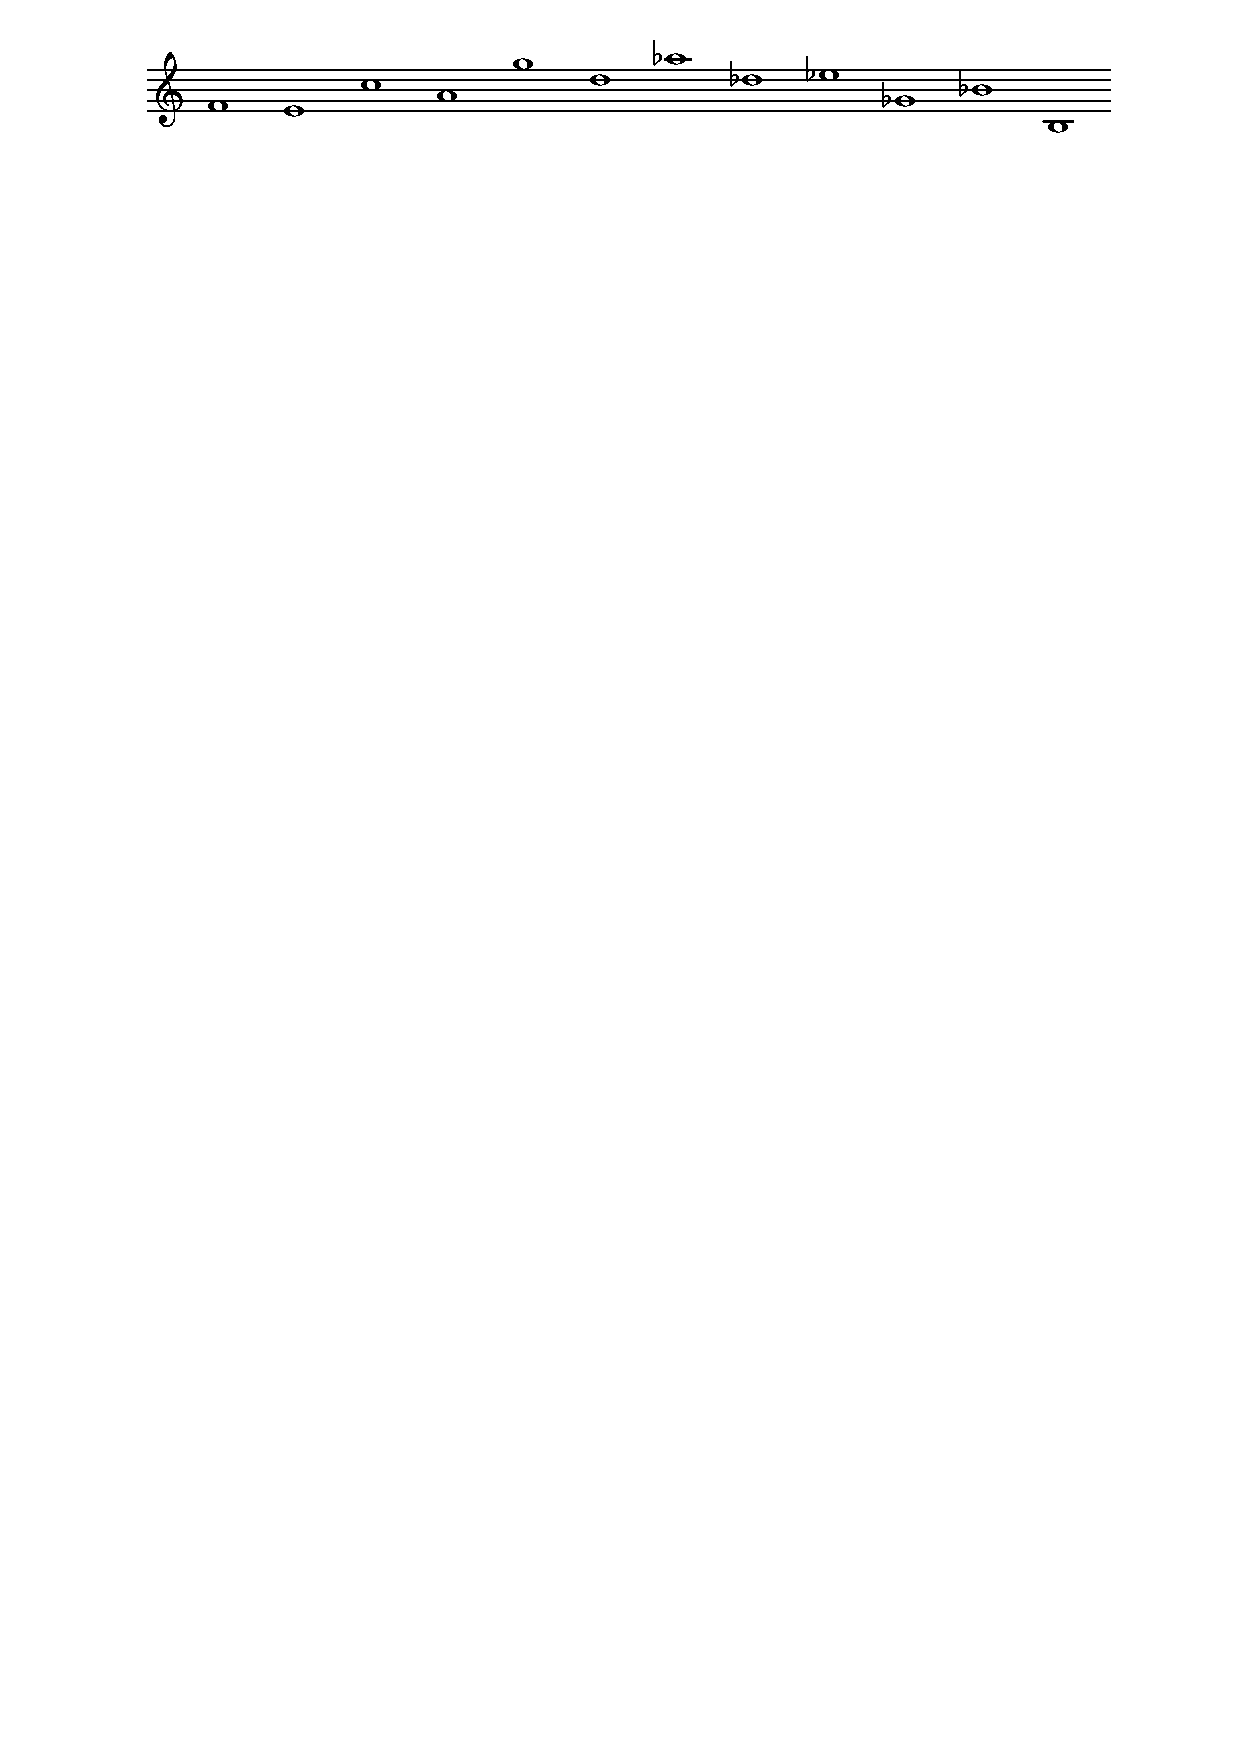
\includegraphics[width=\columnwidth]{imgs/background/serial.pdf}
 \caption{Tone row used by Alban Berg in the \textit{Lyric Suite} for string quartet composed in 1926.}
 \label{fig:serial}
\end{figure}

Table \ref{tab:serial} shows different transformations that can be applied to the tone
row showed in Figure \ref{fig:serial}. The first row, when read from left to right, is the tone row.
When read from right to left, the first row is the retrograde form of the tone row.
The inversion of the tone row is the first column when read from top to bottom.
The retrograde inversion is found by reading the first column from bottom to top.
Each row and column is labeled with $T_i$, where $0 \leq i \leq 11$. A label
$T_i$ means that the respective row is the transposition of the tone row
by $i$ half steps. For example, T5 means the tone row has been
transposed up five half steps from the original form (e.g. a Perfect Fourth).

\begin{table}[h]
    \centering
    % \setlength{\tabcolsep}{4pt}
    \begin{tabular}{ccccccccccccc}
    & T0 & T11 & T7 & T4 & T2 & T9 & T3 & T8 & T10 & T1 & T5 & T6 \\
    \midrule
    T0  & F  & E & C  & A  & G  & D  & Ab & Db & Eb & Gb & Bb & B \\
    T1  & Gb & F & Db & Bb & Ab & Eb & A  & D  & E  & G  & B  & C \\
    T5  & Bb & A & F  & D  & C  & G  & Db & Gb & Ab & B  & Eb & E \\
    T8  & Db & C & Ab & F  & Eb & Bb & E  & A  & B  & D  & Gb & G \\
    T10 & Eb & D & Bb & G  & F  & C  & Gb & B  & Db & E  & Ab & A \\
    T3  & Ab & G & Eb & C  & Bb & F  & B  & E  & Gb & A  & Db & D \\
    T9  & D  & Db & A  & Gb & E & B  & F  & Bb & C & Eb  & G & Ab \\
    T4  & A  & Ab & E  & Db & B & Gb  & C  & F & G & Bb  & D & Eb \\
    T2  & G  & Gb & D  & B  & A  & E  & Bb & Eb & F  & Ab & C & Db \\
    T11 & E  & Eb & B  & Ab & Gb & Db & G  & C  & D  & F  & A & Bb \\
    T7  & C  & B  & G  & E  & D  & A  & Eb & Ab & Bb & Db & F & Gb \\
    T6  & B  & Bb & Gb & Eb & Db & Ab & D  & G  & A  & C  & R & F\\
    \bottomrule
    \end{tabular}
    \caption{Different transformations that can be applied to the tone row showed in Figure \ref{fig:serial}.}
    \label{tab:serial}
\end{table}

% Xenakis
In the 20th century, Iannis Xenakis deeply explored the use of statistical methods to compose \textit{stochastic music} \cite{xenakis1992formalized} -- music in which some elements of the composition are defined randomly. For example, in \textit{Pithoprakta} (1956), he used Gaussian distributions to define the ``temperatures'' of massed glissandi\footnote{Continuous transition between two notes of different pitches.}. In \textit{Achorripsis} (1957), he used Poisson's distribution of rare events to organize ``clouds'' of sound \cite{ames1987automated}. John Cage is another important composer of the 20th century who worked with stochastic music. Cage's \textit{Music of Changes} is a piece for solo piano which was composed using the \textit{I Ching}, a Chinese classic text that is commonly used as a divination system. The I Ching was applied to randomly generate charts of pitches, durations, dynamics, tempo, and densities.

\section{Computational Methods}

% As showed in this section, procedures and rules have been used for centuries to guide different
% aspects of music composition.
% Although many of the procedures presented in the previous section could be
% implemented in a computer, they were not originally designed as computer algorithms.
% The next section presents a short survey of computational methods in AMC.
% ILLIAC Suite (Hiller and Isaacson)
The \textit{ILLIAC Suite: String Quarter No 4} \cite{hiller1957musical}, a composition for string quartet, is considered to be the first music piece to be entirely generated by a digital computer. This piece was generated in 1956 by an ILLIAC computer programmed by Lejaren Hiller and Leonard Isaacson at the University of Illinois. The \textit{ILLIAC Suite} has four movements with melodies that increase in complexity across the movements. The first movement used counterpoint rules from the Renaissance to generate ``simple'' polyphonic melodies. The second movement used a random chromatic method that explored aesthetic differences between seventeenth and twentieth-century musical styles. For the third and fourth movements, Hiller and Isaacson manually designed a Markov chain to generate melodies with the style of Arnold Schoenberg's twelve-tone music.

% Xenakis and John Cage
Xenakis and Cage were also pioneers in the use of computer algorithms to compose music. In 1962, Xenakis wrote the \textit{Stochastic Music Program} in the FORTRAN programming language, which employed probability functions to determine the global structure (e.g. length of sections, density) and the note parameters (e.g. pitch, duration) of his compositions \cite{luque2009stochastic}. \textit{Morsima-Amorsima} is an example of piece composed by Xenakis with the support of this program. From 1967 to 1969, John Cage partnered with Lejaren Hiller to compose a multi-media piece called \textit{HPSCHD}. HPSCHD used a dice game approach where the pre-composed snippets of music were extracted from pieces from Mozart, Beethoven, Chopin, and others.  There are several other early examples of computational approaches to AMC, such as the \textit{Push Button Bertha} \cite{ames1987automated}, a piece generated in 1956 by a DATATRON computer which was programmed by Martin Klein and Douglas Bolitho at the company Burroughs, Inc. Another important early example is the PROJECT1 (1964), a computer program written by Gottfried Michael Koenig that used serial composition and Markov chains to compose pieces such as the \textit{Project 1, Version 1} for 14 instruments.

Most of these early computational examples of AMC were developed by artists in an \textit{ad hoc} way. More recently, computer scientists and engineers started to explore AMC more systematically and a wide range of methods have been proposed: expert systems \cite{gill1963technique}, generative grammars \cite{cope1989experiments}, cellular automata \cite{miranda1993cellular}, evolutionary algorithms \cite{horner1991genetic}, Markov chains \cite{hild1992harmonet}, neural networks \cite{todd1989connectionist}, and others. The remainder of this chapter briefly introduces these methods, except neural networks, which are discussed in great detail in the next chapter.
% Symbolic, Knowledge-Based System
% TODO: rephrase final part

\vspace{0.1in}
\noindent
\textbf{Expert Systems}

\noindent
AMC expert systems use rules that manipulate symbolic music to mimic the reasoning of music composers. For example, Gill \cite{gill1963technique} presented the first application of hierarchical search with backtracking to guide a set of compositional rules from Schoenberg’s twelve-tone technique. Many different works formulated AMC as a \textit{constraint satisfaction problem} (CSP) \cite{anders2011constraint}. For example, Ebcio{\u{g}}lu \cite{ebciouglu1988expert} designed a system called CHORAL for harmonizing four-part chorales in the style of J.S. Bach. The system contains over 270 rules (related to melody, harmony, etc.), expressed in the form of first-order predicate calculus. CHORAL harmonizes the chorales using an informed search method where the heuristics guide the search towards Bachian cadences\footnote{A cadence is a chord progression that occurs at the end of a phrase. A phrase is a series of notes that sound complete even when played apart from the main song.}. Expert systems can also be formalized with \textit{case-based reasoning}. Pereira et al. \cite{pereira1997composing} proposed a system with a case database from just three Baroque music pieces, which were analyzed into hierarchical structures. The system composes just the soprano melodic line of the piece by searching for similar cases in its case database.

% Grammars
% TODO: rephrase final part
\vspace{0.1in}
\noindent
\textbf{Generative Grammars}

\noindent
\textit{Generative grammars} are a set of expansion rules that give instructions for how to expand symbols from a vocabulary. Starting with an initial sequence of symbols, one can compose music with generative grammars by recursively applying expansion rules until a terminal symbol has been reached or a desired length of music has been generated \cite{holtzman1981using}. The expansion rules can be manually defined or inferred from analyzing a corpus of pre-existing music compositions. Lidov and Gadura \cite{lidov1973melody} presented an early example of generative grammar manually designed for the generation of melodies with different rhythmic patterns. A more recent example is the work of Keller and Morrison \cite{keller2007grammatical}, who designed a probabilistic generative grammar for the automatic generation of convincing jazz melodies. In this case, the expansion rules have probabilities associated with them. One of the most famous examples of generative grammars in AMC is Cope's \textit{Experiments in Musical Intelligence} (EMI) \cite{cope1989experiments}, which automatically derives a special type of grammar called \textit{Augmented Transition Network} from a corpus of compositions in a specific style. EMI extracts this augmented transition network by finding short musical patterns that are characteristic of the style being analyzed. EMI also determines how and when to use these patterns in compositions with that style. The inferred transition network can be used to generate new music pieces with the style of the analyzed corpus.

% Self-similarity and Cellular Automata
\vspace{0.1in}
\noindent
\textbf{Cellular Automata}

\noindent
\textit{Cellular Automata} (CA) is a dynamic system composed of simple units (called \textit{cells}) usually arranged in an n-dimensional grid. A cell can be in one state at a time. At each time step, the CA updates each cell according to \textit{transition rules}, which consider the state of the cell and/or the state of the neighbor cells \cite{wolfram2002new}. In his 1986 work \textit{Horos}, Xenakis designed a CA to produce harmonic progressions and new instrument combinations \cite{solomos2005cellular}. CAMUS \cite{miranda1993cellular} is a system that combined two bi-dimensional CAs to compose polyphonic music: Conway's \textit{Game of Life} \cite{gardner1970} and Griffeath’s \textit{Crystalline Growths} \cite{dewdney1989}. Each activated cell in the Game of Life was mapped to a \textit{triad}\textit{A tuple of three notes.}, whose instrument was selected according to the corresponding cell in the Crystalline Growths CA. WolframTones \cite{ball2005making} is a commercial system that composes music with one-dimensional CAs that resemble a selected musical style. The system allows users to select a pre-defined music style (e.g. classical, ambient, jazz) and set different parameters of the algorithm (e.g. rule number, rule type, seed). Moreover, users can define how to map the CA patterns to different musical features (e.g. pitch, tempo, timber).

% Evolutionary
\vspace{0.1in}
\noindent
\textbf{Evolutionary Algorithms}

\noindent
\textit{Evolutionary Algorithms} (EAs) are optimization algorithms that keep a population of candidate solutions (called \textit{individuals}) to maximize (or minimize) a given objective function (called \textit{fitness function}) with a iterative process: (a) evaluation of the current population with the given fitness function, (b) selection of the best solutions and (c) generation of new solutions from the current. Horner and Goldberg \cite{horner1991genetic} presented one of the first examples of EA for music composition. Their algorithm was inspired by a composition technique called \textit{thematic bridging}, where the beginning and end of a piece are given, and a fixed number of transformations (e.g. transposition, inversion, retrograde, etc) are applied to map the beginning into the ending. Each candidate solution was encoded as a fixed set of transformations. The fitness function measured the distance between the ending generated by the candidate and the given ending. New solutions are generated with regular mutation and 1-point crossover. Other examples of EAs are the works of McIntyre \cite{mcintyre1994bach} for four-part baroque harmonization, Polito et al. \cite{polito1997musica} for counterpoint composition, and Papadopoulos and Wiggins \cite{papadopoulos1998genetic} for the generation of melodies for given jazz chord progressions.

Formulating good fitness functions is one of the major challenges of applying evolutionary algorithms for AMC. To deal with this problem, a wide range of works use human evaluators to listen and judge the fitness of the candidate solutions. These approaches are called musical Interactive Genetic Algorithms (IGAs). For example, GenJam \cite{biles1994genjam} is a IGA for generating jazz solos with two hierarchically structured populations: one for bar units and the other for jazz phrases (constructed as sequences of measures). A human evaluator defines the fitness of the candidate solutions with a binary score (good or bad). GenJam accumulates these scores to select phrases during the evolutionary process and generate the solos for a given chord progression. Other examples are presented in the works of Jacob \cite{jacob1995composing}, Schmidl \cite{schmidl2008pseudo}, Tokui and Iba \cite{tokui2000music},
and many others.

\vspace{0.1in}
\noindent
\textbf{Markov Chains}

\noindent
\textit{Markov chains} were a very popular method in the early days of AMC \cite{ames1989markov}.
A Markov chain is a system with a sequence of states, using conditional probabilities to model the transitions between successive states \cite{gillick2010machine}. In a first-order Markov chain, the probability of the next state depends only on the current state, but in an nth-order Markov chain, the probability is conditioned on the previous n-1 states \cite{gillick2010machine}. Markov Chains can be represented as a directed graph where nodes represent states, edges represent transitions between states, and edge weights represent the probability transition between states. This graph can be mapped to a probability table $T$ where rows $i$ and columns $j$ represent nodes, and elements $T_{i,j}$ represent the probability of transitioning between nodes $i$ and $j$. Figure \ref{fig:markov_chain} shows an example of a simple abstract Markov Chain.

\begin{figure}[!h]
 \centering
 \begin{minipage}{0.5\columnwidth}
  \centering
 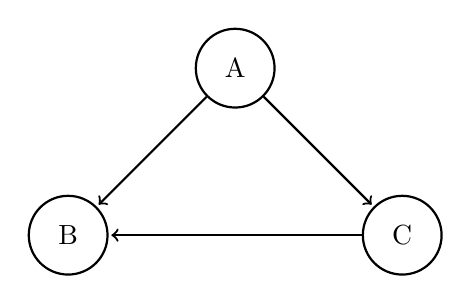
\begin{tikzpicture}[->,shorten >=1pt,auto,node distance=3cm,
         thick,main node/.style={circle,draw,minimum size=1cm,inner sep=0pt]}]

     \node[main node] (A) {A};
     \node[main node] (B) [below left of=A]  {B};
     \node[main node] (C) [below right of=A] {C};

     \draw[->] (A) -- (B);
     \draw[->] (A) -- (C);
     \draw[->] (C) -- (B);
 \end{tikzpicture}
 \end{minipage}
 \begin{minipage}{0.4\columnwidth}
 \centering
 \begin{tabular}{cccc}
   & A   &  B  & C   \\
 \toprule
 A & 0.0 & 0.1 & 0.9 \\
 B & 0.1 & 0.0 & 0.9 \\
 C & 0.5 & 0.5 & 0.0 \\
 \bottomrule
 \end{tabular}

 \end{minipage}

 \caption{Example of Markov Chain represented as a directed.}
 \label{fig:markov_chain}
\end{figure}

Markov chains can be derived manually with the support of music theory  or learned from a corpus of music pieces. In both cases, one has to define how to encode music symbols into a sequence of states \cite{ames1989markov}. To learn a Markov chain from a corpus, one can count, for each state $s_1$ in the corpus, the number of times $s_1$ appears after each other state $s_2$. The transition probability table can then be constructed by normalizing these counts with the total number of transitions in the corpus.
The third and fourth movements of the \textit{ILLIAC Suite} are the earliest examples of
manually-designed Markov chains, while Brooks et al. \cite{brooks1957} presented one of the first examples inferred from a corpus of music. Brooks et al. experimented with different orders of Markov chains where each state represents a pitch class. The probability tables of these chains were learned from thirty-seven common meter ($\frac{4}{4}$) hymn tunes (monophonic). While Markov chains designed manually by composers
worked well for specific compositional tasks \cite{tipei1975mp1, jones1981compositional, langston1989six},
those learned from a corpus, in practice, can capture only short-term dependencies in music
\cite{moorer1972music}. Moreover, low order chains typically generate unmusical compositions that
wander aimlessly, while high order ones tend to repeat segments from the corpus and are
very expensive to train \cite{moorer1972music}.

Markov chains can also be used to evaluate music generated by other methods. Given a sequence of states representing a piece of music, one can evaluate this piece with the joint probability of the sequence as given by the Markov chain. Thus, the higher the probability, the better the music. This approach was used by Lo and Lucas \cite{lo2006evolving}. They trained a Markov chain with classical music pieces and used it to calculate the fitness of candidate solutions of an EA. Each solution in the EA represents a melody encoded as a sequence of pitch numbers as defined by the MIDI format.

% TODO: Conclude this chapter linking markov chains with deep learning
Most of methods presented in this section require musical models (or rules) to be defined and encoded
to manipulate or evaluate music. Although music theory formalizes several aspects of music analysis and composition, defining and encoding computational music models for AMC is still very challenging, given that music composition is a creative task. Some of the presented methods, such as generative grammars and Markov models, can infer these rules from a corpus of music. However, in practice, they have shown to have limited performance in terms of music quality. Deep learning is a modern approach to AI, where neural networks are trained to perform various tasks. Recently, the AI research community has drawn strong attention to this approach due to the impressive results that it has been achieving in different problems
(e.g. image classification, speech recognition, and machine translation) \cite{lecun2015deep}. These results also motivated AMC researchers to explore deep learning algorithms for music composition \cite{briot2017deep}. The next chapter presents a detailed discussion on how deep learning can be used to learn music rules from a corpus of pieces.
